\documentclass{standalone}
\usepackage{pgfplots}
\usetikzlibrary{arrows.meta} 
\pgfplotsset{compat=1.18}
\begin{document}
	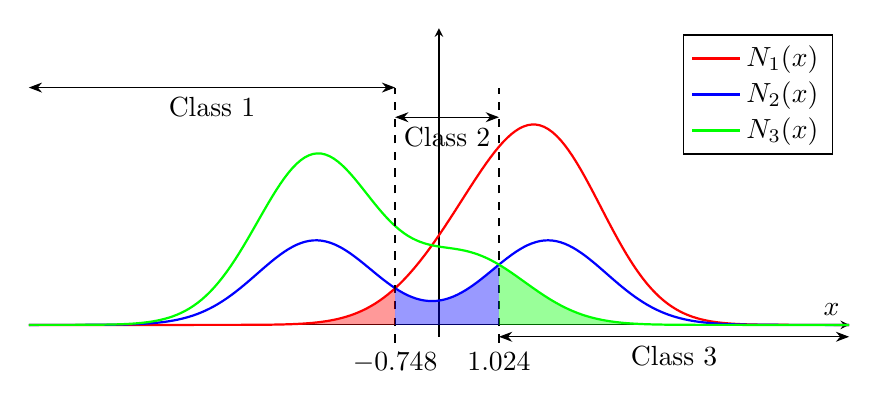
\begin{tikzpicture}
		\begin{axis}[
			domain=-7:7,
			samples=200,
			axis lines=middle,
			xlabel={$x$},
			xtick=\empty,
			ytick=\empty,
			ymin=-0.02, ymax=0.5,
			enlargelimits=false,
			clip=false,
			grid=major,
			width=12cm, height=5.5cm
			]
			
			\def\sigma{1}
			\def\xa{-0.748}
			\def\xb{1.024}
			
			% Normal mixture curves
			\addplot[red, thick]
			{4/14*1/(\sigma*sqrt(2*pi)) * exp(-((x-0.5)^2)/(2*\sigma^2))+10/14*1/(\sigma*sqrt(2*pi)) * exp(-((x-1.86)^2)/(2*\sigma^2))};
			\addlegendentry{$N_1(x)$}
			
			\addplot[blue, thick]
			{5/14*1/(\sigma*sqrt(2*pi)) * exp(-((x+2.1)^2)/(2*\sigma^2))+5/14*1/(\sigma*sqrt(2*pi)) * exp(-((x-1.86)^2)/(2*\sigma^2))};
			\addlegendentry{$N_2(x)$}
			
			\addplot[green, thick]
			{10/14*1/(\sigma*sqrt(2*pi)) * exp(-((x+2.1)^2)/(2*\sigma^2))+4/14*1/(\sigma*sqrt(2*pi)) * exp(-((x-0.5)^2)/(2*\sigma^2))};
			\addlegendentry{$N_3(x)$}
			
			% vertical dashed decision boundaries (as in your original)
			\addplot[black, dashed, thick] coordinates {(\xa,-0.03) (\xa,0.4)};
			\node[below] at (axis cs:\xa,-0.03) {$-0.748$};
			
			\addplot[black, dashed, thick] coordinates {(\xb,-0.03) (\xb,0.4)};
			\node[below] at (axis cs:\xb,-0.03) {$1.024$};
	
			\fill [red, opacity = .4, domain=-7:-0.748, variable=\x]
			(-7, 0)
			-- plot ({\x}, {4/14*1/(\sigma*sqrt(2*pi)) * exp(-((\x-0.5)^2)/(2*\sigma^2))+10/14*1/(\sigma*sqrt(2*pi)) * exp(-((\x-1.86)^2)/(2*\sigma^2))})
			-- (-0.748, 0)
			-- cycle;
			\fill [blue, opacity = .4, domain=-0.748:1.024, variable=\x]
			(-0.748, 0)
			-- plot ({\x}, {5/14*1/(\sigma*sqrt(2*pi)) * exp(-((\x+2.1)^2)/(2*\sigma^2))+5/14*1/(\sigma*sqrt(2*pi)) * exp(-((\x-1.86)^2)/(2*\sigma^2))})
			-- (1.024, 0)
			-- cycle;
			\fill [green, opacity = .4, domain=1.024:7, variable=\x]
			(1.024, 0)
			-- plot ({\x}, {10/14*1/(\sigma*sqrt(2*pi)) * exp(-((\x+2.1)^2)/(2*\sigma^2))+4/14*1/(\sigma*sqrt(2*pi)) * exp(-((\x-0.5)^2)/(2*\sigma^2))})
			-- (7, 0)
			-- cycle;

			\draw[Stealth-Stealth] (-0.748,0.4) -- (-7,0.4)
			node[midway, below] {Class 1};

			\draw[Stealth-Stealth] (-0.748,0.35) -- (1.024,0.35)
			node[midway, below] {Class 2};
			
			\draw[Stealth-Stealth] (7,-0.02) -- (1.024,-0.02)
			node[midway, below] {Class 3};
		\end{axis}
	\end{tikzpicture}
\end{document}
